  \documentclass[a4paper]{article}
\linespread{1.5}
\usepackage[round]{natbib}
\usepackage{amssymb, amsmath}
%% \usepackage{RJournal}
\usepackage{fancyvrb}
\usepackage{Sweave, url, tikz}
\usepackage{hyperref}
\usepackage[sc]{mathpazo}
\usepackage[T1]{fontenc}
\usepackage{geometry}
\geometry{verbose,tmargin=2.5cm,bmargin=2.5cm,lmargin=2.5cm,rmargin=2.5cm}
\setcounter{secnumdepth}{2}
\setcounter{tocdepth}{2}
\usepackage{url}
\usepackage{breakurl}
\usepackage[utf8]{inputenc}

\newcommand{\ts}{\textsuperscript}
\newcommand\bc{\begin{center}}
\newcommand\ec{\end{center}}

\DefineVerbatimEnvironment{Sinput}{Verbatim}{fontsize=\small,fontshape=sl}
\DefineVerbatimEnvironment{Soutput}{Verbatim}{fontsize=\small}
\DefineVerbatimEnvironment{Scode}{Verbatim}{fontsize=\small,fontshape=sl}
\fvset{listparameters={\setlength{\topsep}{0pt}}}
\renewenvironment{Schunk}{\vspace{\topsep}}{\vspace{\topsep}}



\bibliographystyle{abbrvnat}

\begin{document}
\Sconcordance{concordance:CDS.tex:CDS.Rnw:%
1 138 1 1 4 1 2 1 0 1 7 9 0 1 2 70 1 1 5 7 0 1 2 134 1 1 2 12 0 1 2 150 1 1 2 1 0 1 1 6 0 %
1 2 5 1 1 2 4 0 1 2 10 1 1 2 34 0 1 2 46 1 1 2 4 0 1 2 4 1 1 2 23 0 1 2 3 1 1 2 13 0 1 2 %
55 1}

\title{A Guide to the CDS Package}
\author{Heidi Chen\thanks{\href{mailto:s.heidi.chen@gmail.com}{s.heidi.chen@gmail.com}}, David Kane\thanks{\href{mailto:dave.kane@gmail.com}{dave.kane@gmail.com}}, and Yang Lu\thanks{\href{mailto:yang.lu2014@gmail.com}{yang.lu2014@gmail.com}}}
\maketitle

%%\VignetteIndexEntry{Using the CDS package}
%%\VignetteDepends{CDS}

\setkeys{Gin}{width=0.95\textwidth}


\section{Introduction}

%% 1 paragraph

A Credit Default Swap (CDS) is an agreement between two
counterparties in which the buyer pays a fixed periodic coupon to the
seller in exchange for protection in the case of a credit event. The
International Swaps and Derivatives Association (ISDA) has created a
set of standard terms for CDS contracts, the so-called ``Standard
Model.'' This allows market participants to calculate cash settlement
from conventional spread quotations, convert between conventional
spread and upfront payments, and build the spread curve of a CDS. The
\textbf{CDS} package implements the Standard Model, allowing users to
value credit default swaps and calculate various risk measures
associated with these instruments.

%% Are the "standard terms for CDS contracts" really the same thing as the 
%% Standard Model? I am not so sure. I think that the standard terms are 
%% things like XR and MM, strict definitions for credit events, auction
%% proceedures and so on. I think that the Standard Model just refers to the
%% math. But perhaps this is too confusing a distinction (and I might be 
%% wrong), so leave it for the next version.

%% By the way, I am thinking that a good target journal for this piece may be
%% The Journal of Statistical Software. If so, we can/should make this much
%% longer than it currently is, including getting a lot of the details correct,
%% which is why I am adding these notes.

\section{CDS Basics}
\label{sec:CDSBasics}

%% what's a CDS

A CDS is a simple and popular form of credit derivative. It was
originated in the late 1980s and was popularized by a team at
J.P. Morgan including Blythe Masters.\citep{cdsOrigins,
  blythe} The CDS market started to develop soon afterwards as banks
used CDS contracts to hedge the credit exposures on their balance
sheets. Many different types of CDS have since emerged including
basket default swaps (BDSs), index CDSs, credit-linked notes, et
cetera \citep{jk}. In the \textbf{CDS} package, we focus on calculations
related to a single-name, or corporate, credit default swaps.

%% mechanics of a single-name CDS contract

%% Might be good to expand this with a specific example. Use a real CDS
%% (with a name, termination date and so on) and give the details of
%% the bond that is the reference obligation. Cite the Markit webpage.
%% Leave nothing out.

A single-name CDS contract provides a transfer of credit risk between
two parties. The buyer of a CDS contract (protection buyer) transfers
the credit risk to the CDS seller (protection seller) by paying a
series of coupons until the contract terminates. In other words, the
protection buyer is short credit by selling the credit risk of an
underlying bond to the protection seller. As shown in Figure
\ref{fig:cashFlow}, the buyer pays a stream of coupon payments, called
the premium leg, in order to receive a one-time, contingent payment,
called the protection leg, in the case of a credit event. A credit
event triggers the settlement under a CDS contract. Possible credit
events include banruptcy and debt restructing. The exact definition
varies among CDS contracts.\\

%% Define XR and MM in the next version.

%% Might add some more details. Or, better, use one of the images from
%% Barclays or Bloomberg, citing them of course.

\begin{figure}
  \caption{\label{fig:cashFlow} Mechanics of a CDS contract}
\begin{center}
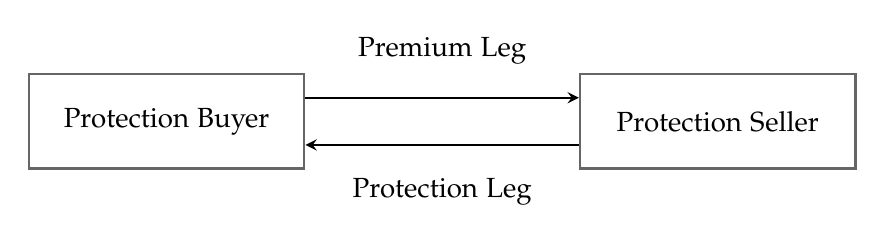
\begin{tikzpicture}[
squarednode/.style={rectangle, draw=black!60, fill=none, thick, 
  minimum height =12mm, minimum width = 35mm},
]
  \tikzset{mylabel/.style = {text centered}
  }

\vspace{2cm}
    \node [squarednode](A) at (0,0) {Protection Buyer};
    \node [squarednode](B) at (7,0) {Protection Seller};

    \draw[transform canvas={yshift=3mm},-stealth, thick] (A) -- (B);
    \draw[transform canvas={yshift=-3mm},-stealth, thick] (B) -- (A);
    \node[mylabel] at (3.5, 0.9) {Premium Leg};
    \node[mylabel] at (3.5, -0.9) {Protection Leg};
    
\end{tikzpicture} 
\end{center}
\end{figure}

In the \textbf{CDS} package, we call the function \texttt{CDS} to
construct an object of a class \texttt{CDS}. Below we show an example
of how to construct a CDS contract in the package.


\begin{Schunk}
\begin{Sinput}
> library(CDS)
> cds1 <- CDS(entityName = "IBM",
+             RED = "49EB20",
+             TDate = "2014-04-15",
+             maturity = "5Y",
+             notional = 1e7,
+             coupon = 100,
+             parSpread = 50)
\end{Sinput}
\end{Schunk}


%% In the next draft, we should not have a clunky list of terms.
%% Better to introduce the terms, bolding them the first time
%% they appear, in a discussion of a specific CDS. 

%% Start with a bond portfolio manager who owns a specifi bond,
%% something that is a reference obligation for a member of CDX IG. 
%% That PM is concerned about the credit worthiness of the company,
%% at least over the next year or two. But selling the bond is too
%% expensive or annoying. So, he can buy some CDS protection on 
%% the bond. And so on. Describe all the cash flows, both from his
%% point of view, and the point of view of the hedge fund that sells
%% the protection. Better yet, have the exercise occur in the past,
%% but use a bond that actually defaulted. Then we can talk about the
%% auction, recovery rate and so on.

As shown in the example, a CDS contract between two counterparties
typically specifies the following key terms:\footnote{Some of the
  definitions come from \textit{Credit Derivatives Glossary}
  \citep{glossary}, \textit{Standard Corporate CDS Handbook}
  \citep{barclays}, \textit{Credit Derivatives} \citep{bloomberg}, and
  \textit{The Pricing and Risk Management of Credit Default Swaps,
    with a Focus on the ISDA Model} \citep{openGamma}.}
\begin{description}
\item[Reference Entity] refers to the legal entity which is the
  subject of a CDS contract. \texttt{entityName} in the \texttt{CDS}
  function takes the name of the legal entity and is ``IBM'' in
  \texttt{cds1}.
\item [RED] is a Markit product. It stands for Reference Entity
  Database. Each entity/seniority pair has a unique 6 digit RED
  code. Each deliverable bond has a 9 digit RED code, the first 6
  digits of which matches the 6 digit code of the associated
  entity/seniority. Each entity also has a ``preferred reference
  obligation'' that is the default reference obligation for CDS
  trades. A user can input either the six-digit RED code or the
  nine-digit RED pair code. The input ``49EB20'' is the six-digit RED
  code for ``IBM''.
\item [Trade Date] or \textbf{TDate} as shown in the argument of the
  \texttt{CDS} function indicates the trade date of the CDS contract
  and is April 15, 2014 in \texttt{cds1}.
\item[Maturity] refers to the fixed date on which a CDS contract
  terminates. However, speaking colloquially, it can also be the
  length of time remaining until that date. This length is also called
  the \textbf{tenor} of a CDS contract. The most commonly traded CDS
  are the 5 years. The protection buyer continues to make payments to
  the protection seller till maturity of the contract or the
  occurrence of a credit event. The maturity is 5 years in
  \texttt{cds1}.
\item[Notional] is the amount of the underlying asset on which the
  payments are based. It is \$10 million in \texttt{cds1}.
\item[Coupon] is quoted in basis points. It specifies the payment
  amount from the protection buyer to the seller on an annual
  basis. Coupons are paid quarterly. This contract has a coupon of 100
  bps.
\item[Spread] is quoted in basis points per year. If, instead of using
  a fixed coupon and exchanging upfront fees, the buyer and seller of
  protection were to agree on a variable coupon, then the spread is
  the coupon size that they would agree on. It is quoted as 50 bps in
  \texttt{cds1}.
\end{description}


Here the user enters the CDS contract with ``IBM'' as the underlying
entity and sets the spread at 50 bps and the coupon at 100
bps. However, the valuation of a CDS contract requires neither the
entity name or the RED Code. She does not have to know the information
to use the package. As shown below, insofar as she inputs the same
\texttt{TDate}, \texttt{parSpread}, and \texttt{maturity} information,
the valuation of the contract will be the same.

\begin{Schunk}
\begin{Sinput}
> cds2 <- CDS(TDate = "2014-04-15",
+             maturity = "5Y",
+             coupon = 100,
+             parSpread = 50)
\end{Sinput}
\end{Schunk}


Besides \texttt{parSpread}, a market paricipant can choose to specify
either \texttt{ptsUpfront} or \texttt{upfront} to construct a
\texttt{CDS} class object.\footnote{See Section \ref{sec:isda} for
  definitions on both terms.} \texttt{ptsUpfront} or \texttt{upfront}
refer to points upfront (in \%), and upfront payment (in dollar
amount) of a CDS contract, respectively. One of the three arguments
has to be specified in order to construct the \texttt{CDS} class
object.


\section{The ISDA Standard Model}
\label{sec:isda}
%% the origins of the ISDA standard model. Next version: Talk about Europe?

In April 2009 in North America, ISDA introduced a series of mandatory
modifications to the CDS contract known as the ``Big Bang Protocol.''
Among these changes were the standardization rules on the first
accrual dates, fixed coupon rates (100 bps or 500 bps), and the
recovery rate (40\%).

%% specifications of the ISDA standard CDS contract

An ISDA standard CDS contract specifies the following:\footnote{Refer
  to the \textit{ISDA Standard CDS Converter Specification} for
  details.}
\begin{description}
\item[Trade Date] refers to the date of the trade.
\item[Maturity] is the length of the contract. The most commonly traded
  contracts have a maturity of 5 years.
\item[Maturity Date] falls on one of the four dates (Mar/Jun/Sep/Dec
  20th) in a year. One can add the maturity of the contract to the
  trade date; the next available date among those four dates is the
  maturity date.
\item[Backstop Date] is the date from which protection is
  provided,
  \begin{center}
    Backstop Date = T - 60 Calender Days.
  \end{center}
\item[Notional Amount] is in millions.
\item[Standard Coupon] is either 100 or 500 bps per
  year for CDS contracts in North America.
  %% , and 25, 100, 500 or 1000 bps in Europe.
\item[Recovery Rate] is the estimated percentage of par value that
  bondholders will receive after a credit event. It is commonly
  reported in percentage of notional value. CDS contracts for corporate bonds
  assume a 40\% recovery rate for valuation purposes. 
\item[Par Spread] is the spread value which makes the present value
  of a CDS contract zero. It is quoted in basis points.  
\item[Upfront Payment] is quoted in the currency amount. Since a
  standard contract is traded with fixed coupons, upfront payment is
  introduced to reconcile the difference in contract value due to the
  difference between the fixed coupon and the par
  spread. There are two types of upfront, dirty and clean. Dirty
  upfront (\textbf{Cash Settlement Amount}) refers to the market
  value of a CDS contract. Clean upfront is dirty upfront less any
  accrued interest payment, and is also called the \textbf{Principal}.
\item[Points Upfront], or simply \textbf{points}, are quoted as a
  percentage of the notional amount. They represent the upfront
  payment excluding the accrual payment. High yield CDS contracts
  are often quoted in points upfront. The protection buyer pays the
  upfront payment if points upfront are positive, and the buyer is
  paid by the seller if the points are negative.
\end{description}

The Standard Model allows market participants to convert between
the par spread and the upfront payment, and compute the cash
settlement amount for a standard contract. A few key assumptions and
definitions used when valuing a Standard CDS contract are the
following:\footnote{Please refer to \url{http://bit.ly/1kg5qPw} for
  more infrmation on the ISDA standard CDS model assumptions.}

%% cds converter specification pdf original
%% url. http://www.cdsmodel.com/assets/cds-model/docs/ISDA\%20Standard\%20CDS\%20Contract\%20Converter\%20Specification\%20-\%20Sept\%204,\%202009.pdf}

\begin{description}
\item[Trade Date (T)] means 11:59pm on the trade date.
\item[Days of Protection] is the number of days
  from Maturity Date to Trade Date.
\item[Mark-to-market (MTM)] represents the contract value to the
  protection buyer. It is computed by discounting the expected
  protection leg and premium leg cashflows to T.
\item[Accrued Premium] is the premium that has accrued from accrual
  begin date to T where both dates are inclusive.
\end{description}

%% http://www.cdsmodel.com/assets/cds-model/docs/Interest%20Rate%20Curve%20Specification%20-%20All%20Currencies%20%28Updated%20May%202013%29.pdf

The ISDA also standardizes the interest rates used by the Standard
Model in valuing a CDS contract. There are two types of rates used in
valuing a USD denominated CDS contract - cash rates and swap
rates. Cash rates are of maturity 1, 2, 3, 6 months, and 1 year. They
are provided by the British Bankers' Association (BBA). Swap rates are
of maturity 2, 3, 4, 5, 6, 7, 8, 9, 10, 12, 15, 20, 25, and 30 years,
and are provided by ICAP \citep{rates}. The Standard Model follows the
conventions below for interpolation of the entire USD yield curve:
\begin{itemize}
\item The day count convention (DCC) for money market instruments and
  floating legs of the swaps is \textbf{ACT/360}.
\item DCC for floating legs of the swaps is \textbf{30/360}.
\item Payment frequency for fixed legs of the swaps is 6 months.
\item Payment frequency for floating legs of the swaps is 3
  months.\footnote{See
    \url{http://www.fincad.com/derivatives-resources/wiki/swap-pricing.aspx}
    for details on floating and fixed legs calculation.}
\item A business day calendar of weekdays (Monday to Friday) is
  assumed. Saturdays and Sundays will be the only non-business days.
\item If a date falls on a non-business day, the convention used for
  adjusting coupon payment dates is \textbf{M} (Modified Following).
\end{itemize}



\section{Using the CDS package}

Currently, a market participant can conduct CDS-related calculations
by using the \textbf{CDSW Calculator} on a Bloomberg Terminal or the
Markit CDS Calculator.\footnote{The Markit CDS Calculator is available
  at \url{http://www.markit.com/markit.jsp?jsppage=pv.jsp}.} The
\textbf{CDS} package provides tools for valuing a single-name CDS
contract. The default setting allows a user to value a USD-denominated
CDS contract following the Standard Model as mentioned in Section
\ref{sec:isda}. She can also specify her own set of parameters to
customize the calculation. We have illustrated the construction of a
CDS contract using the \textbf{CDS} package in previous sections. In
this section, we will demonstrate the use of the \textbf{CDS} package
in more detail and provide a series of examples.

Recall that in Section \ref{sec:CDSBasics}, a \texttt{CDS} class
object called \texttt{cds1} has been constructed. Its maturity is 5
years. Its spread is set at 50 bps and the coupon, 100 bps. The
notional amount is \$10 million. A user can call \texttt{summary} on a
\texttt{cds1} to view essential information on the contract.

\begin{Schunk}
\begin{Sinput}
> summary(cds1)
\end{Sinput}
\begin{Soutput}
Contract Type:                      SNAC   TDate:                     2014-04-15
Entity Name:                         IBM   RED:                           49EB20
Currency:                            USD   End Date:                  2019-06-20
Spread:                               50   Coupon:                           100
Upfront:                        -256,577   Spread DV01:                    5,086
IR DV01:                           66.14   Rec Risk (1 pct):               90.03
\end{Soutput}
\end{Schunk}

%% Biggest flaw of the current version of the paper is that you 
%% do not walk the reader through this specific example. Having shown 
%% this summary, you need to --- now! --- explain each element in the 
%% presentation. Tell us, now, what Spread DV01 of 5,086 means. Don't
%% wait five pages and then not even mention this specific number! If you
%% need to do preliminary work before hand, then, fine, do that work and
%% wait to do the summary.

%% Note that we could use a lot more detail, both before we get to concepts 
%% like recovery rate and in explaining just why they matter.

%% This is very sloppy. First, you should go through everything in the
%% summary item by item. Second, it should be in the same order as the
%% summary. Third, it should use the same lingo. Is "TDate" the same
%% as Trade Date? How am I supposed to know that. Fourth, it should
%% mention the values from the summary.

%% In other words, this section is not about what an "An ISDA standard 
%% CDS contract specifies"! It is about the summary you have just shown.

In the summary output, it shows that the type of the CDS contract is
``SNAC''. \texttt{TDate} refers to the trade date and is April 15,
2014. \texttt{entityName} refers to the entity name of the CDS
contract and is ``IBM''. The \texttt{RED} code is ``48EB20'' as
specified by the user. \texttt{spread} shows that the quoted spread
for the contract is 50 bps and the coupon is 100 bps as shown in the
\texttt{coupon} field. \texttt{upfront} indicates the dirty upfront
payment in dollars or the cash settlement amount. It is -256,577
dollars, which means that from a buyer's perspective, the net present
value of the remaining expected cashflows is -\$256,577.

To understand the remaining three items from the \texttt{summary}
output (\texttt{Spread DV01}, \texttt{IR DV01}, and \texttt{Rec Risk
  (1 pct)}), one needs to understand \textbf{PV01}, an essential
component to the mark-to-market calculation of a CDS contract. PV01 is
the present value of a stream of 1 basis point payments at each CDS
coupon date. It is sometimes referred to as the \textbf{CDS duration}
or \textbf{risky duration}.

Analytically, PV01 can be calculated by
\begin{displaymath}
PV01 =  \sum_tDf(t_i)S(t_i)B(t_i), \nonumber\\
\end{displaymath}
where 
\begin{itemize}
\item $i =$ coupon index,
\item $t_i =$ coupon date,
\item $Df(f_i) =$ discount factor until $t_i$,
\item $S(t_i) =$ survival probability until $t_i$,
\item $B(t_i) =$ day count fraction at $t_i$.
\end{itemize}

We can thus calculate the principal amount (clean upfront payment)
paid from the protection buyer to the seller using the following
formula:
\begin{center}
  Principal Amount = (Par Spread - Coupon) $\times$ PV01.
\end{center}

Using the concept of PV01, we show the calculation of the main risks
(exposures) of a CDS position, \textbf{Spread DV01}. Spread DV01
reflects the risk duration of a CDS trade, also known as \textbf{Sprd
  DV01}, \textbf{Credit DV01}, \textbf{Spread Delta}, and just
\textbf{DV01}. 

It measures the sensitivity of a CDS contract mark-to-market to a
parallel shift in the term structure of the par spread. DV01 should
always be positive for a protection buyer since she is short credit
and a rising spread is a sign of credit deterioration. Starting with
PV01 and taking the derivative with respect to the spread give us:
\begin{eqnarray}
  PV & = & (S - C) * PV01 \nonumber \\
  DV01 & = & \frac{\partial PV}{\partial S} \nonumber \\
  & = & PV01 + (S - C) \frac{\partial PV01}{\partial S},\nonumber
\end{eqnarray}
where $S$ is the spread of the contract and $C$ is the coupon.

Both DV01 and PV01 are measured in dollars and are equal if the spread
equals the coupon. The Spread DV01 of \texttt{cds1} is \$5,086.

\textbf{IR DV01} is the change in value of a CDS contract for a 1 bp
parallel increase in the interest rate curve. IR DV01 is, typically, a
much smaller dollar value than Spread DV01 because moves in overall
interest rates have a much smaller effect on the value of a CDS
contract than does a move in the CDS spread itself. In \texttt{cds1},
the IR DV01 is \$66.14. \textbf{Recovery Risk 01} or \texttt{Rec Risk
  (1 pct)} as shown in the \texttt{summary} output, is the dollar
value change in market value if the recovery rate used in the CDS
valuation were increased by 1\%. It is \$90.03 in \texttt{cds1}.


The default settings of valuing a CDS contract in the \textbf{CDS}
package follow the Standard North American Corporate (SNAC) CDS
Contract specifications.\footnote{See
  \url{http://www.cdsmodel.com/assets/cds-model/docs/Standard\%20CDS\%20Contract\%20Specification.pdf}
  for details.} Below we list the ISDA specifications implemented in
the \textbf{CDS} package. Additional default settings in the package
which are not specified by the Standard Model, such as the default
notional amount, are also listed.

\begin{itemize}
\item Currency: USD.
\item Trade Date (T): the current business day.
\item CDS Date: Mar/Jun/Sep/Dec 20th of a year.
\item Maturity: 5 years.
\item Maturity Date (End Date): It falls on a CDS date without
  adjustment.
\item Coupon Rate: 100 bps.
\item Notional Amount (MM): 10MM.
\item Recovery Rate (\%): 40\% for senior debts.
\item Premium Leg:
  \begin{itemize}
    \item Payment Frequency: quarterly
    \item DCC: ACT/360
    \item Pay Accrued On Default: It determines whether accrued
      interest is paid on a default. If a company defaults between
      payment dates, there is a certain amount of accrued payment that
      is owed to the protection seller. ``True'' means that this
      accrued will need to be paid by the protection buyer, ``False''
      otherwise. The defalt is ``True,''
    \item Adjusted CDS Dates: ``F.'' It means that it assumes the next
      available business day when a CDS date falls on a non-business day
      except the maturity date.
    \item First Coupon Payment: It is the earliest Adjusted CDS Date
      after T + 1.
    \item Accrual Begin Date (Start Date): It is the latest Adjusted
      CDS Date on or before T + 1.
    \item Accrual Period: It is from previous accrual date (inclusive)
      to the next accrual date (exclusive), except for the last
      accrual period where the accrual end date (Maturity Date) is
      included.
  \end{itemize}
\item Protection Leg:
  \begin{itemize}
  \item Protection Effective Date (Backdrop Date): T - 60 calendar
    days for credit events.
  \item Protection Maturity Date: Maturity Date.
  \item Protection Payoff: Par minus Recovery.
  \end{itemize}
\end{itemize}


\subsection{More on CDS pricing}

\texttt{CS10} is a method which calculates the change in value of the
CDS contract when the spread of the contract increases by
10\%. \texttt{CS10} takes in a \texttt{CDS} class object formed by
calling the \texttt{CDS} function. The CS10 of \texttt{cds1} is
\$25385.2.

\begin{Schunk}
\begin{Sinput}
> cds1.CS10 <- CS10(cds1)
> cds1.CS10
\end{Sinput}
\begin{Soutput}
[1] 25385.2
\end{Soutput}
\end{Schunk}

A market participant can also update the \texttt{CDS} class objects she
has constructed by calling the \texttt{update} method. It updates a
\texttt{CDS} class object with a new spread, points upfront or upfront
by specifiying the relevant input.

\begin{Schunk}
\begin{Sinput}
> cds3 <- update(cds1, spread = 55)
\end{Sinput}
\end{Schunk}

\texttt{cds3} is a new \texttt{CDS} class object with a spread of 55
bps; all other specifications of the contract are the same as those in
\texttt{cds1} since it is updated from \texttt{cds1}. One can also
specify \texttt{upfront} (in dollar amount) or \texttt{ptsUpfront} (in
bps) in the \texttt{update} method.

Besides calling the \texttt{summary} method, one can type in the name
of the \texttt{CDS} class object in the current \textbf{R} Session and
obtain a full description of the CDS contract.

\begin{Schunk}
\begin{Sinput}
> cds3
\end{Sinput}
\begin{Soutput}
CDS Contract 
Contract Type:                      SNAC   Currency:                         USD
Entity Name:                         IBM   RED:                           49EB20
TDate:                        2014-04-15   End Date:                  2019-06-20
Start Date:                   2014-03-20   Backstop Date:             2014-02-14
1st Coupon:                   2014-06-20   Pen Coupon:                2019-03-20
Day Cnt:                         ACT/360   Freq:                               Q

Calculation 
Value Date:                   2014-04-18   Price:                         102.24
Spread:                               55   Pts Upfront:                  -0.0224
Principal:                      -223,692   Spread DV01:                    5,064
Accrual:                          -7,500   IR DV01:                        59.35
Upfront:                        -231,192   Rec Risk (1 pct):               88.87
Default Prob:                      0.047   Default Expo:               6,223,692

Credit curve effective of 2014-04-15 
 Term     Rate Term     Rate
   1M 0.001517   7Y 0.022630
   2M 0.001923   8Y 0.024580
   3M 0.002287   9Y 0.026265
   6M 0.003227  10Y 0.027590
   1Y 0.005465  12Y 0.029715
   2Y 0.005105  15Y 0.031820
   3Y 0.009265  20Y 0.033635
   4Y 0.013470  25Y 0.034420
   5Y 0.017150  30Y 0.034780
   6Y 0.020160              
\end{Soutput}
\end{Schunk}

There are three parts of the output. The first part ``CDS Contract''
provides basic information on the contract including ``Contract
Type'', ``Currency'', ``Entity Name'', ``RED'', ``TDate'', various
dates related to the contract, and the day count conventions for
\texttt{cds3}. 

The second part of the output contains relevant risks measures of
\texttt{cds3}. \texttt{Price} refers to the clean dollar price of the
contract and is calculated by
\begin{equation}
  \begin{aligned}
    {\rm Price} & =  (1 - {\rm Principal} / {\rm Notional})*100  \nonumber \\
    & =  100 - \text{Points Upfront}. \nonumber
  \end{aligned}
\end{equation}

The price of \texttt{cds3} is 102.24, greater than 100. A CDS will
have a price greater than 100 if the points upfront are negative, that
is, the CDS buyer needs to receive money to obtain protection because
he promises to pay a coupon of, say, 100 even if the spread is
60. This is analogous to a bond investor paying more than the face
value of a bond because current interest rates are lower than the
coupon rate on the bond.

``Default Prob'' refers to the default probability which is the
estimated probability of default for each maturity by a given time. It
can be approximated by
\begin{equation}
  \text{Default Prob} \approx \left [1 - exp \left (\frac{rt}{1-R} \right ) \right ], \nonumber
\end{equation}
where $r$ is the spread, $t$ is the time to maturity, and $R$ is the
recovery rate. The default probability for \texttt{cds3} is 4.7\%.

``Default Expo'' refers to the expoure to the default of a CDS
contract based on the formula below.
\begin{equation}
  \text{Default Exposure} = (1 - \text{Recovery Rate})*\text{Notional}
  - \text{Principal}. \nonumber
\end{equation}

The last part of the output reports the interest rates used in the
calculation.

Calling the function \texttt{getRates} also produces the rates used in
building a curve for CDS valuation. 

\begin{Schunk}
\begin{Sinput}
> cds3Rates <- getRates(date = "2014-04-15")
\end{Sinput}
\end{Schunk}

The output consists of two list objects. The first list contains rates
of various maturities. They are directly obtained from the Markit
website based on the specifications \citep{rates}.

\begin{Schunk}
\begin{Soutput}
   expiry matureDate     rate type
1      1M 2014-05-19 0.001517    M
2      2M 2014-06-17 0.001923    M
3      3M 2014-07-17 0.002287    M
4      6M 2014-10-17 0.003227    M
5      1Y 2015-04-17 0.005465    M
6      2Y 2016-04-17 0.005105    S
7      3Y 2017-04-17 0.009265    S
8      4Y 2018-04-17  0.01347    S
9      5Y 2019-04-17  0.01715    S
10     6Y 2020-04-17  0.02016    S
11     7Y 2021-04-17  0.02263    S
12     8Y 2022-04-17  0.02458    S
13     9Y 2023-04-17 0.026265    S
14    10Y 2024-04-17  0.02759    S
15    12Y 2026-04-17 0.029715    S
16    15Y 2029-04-17  0.03182    S
17    20Y 2034-04-17 0.033635    S
18    25Y 2039-04-17  0.03442    S
19    30Y 2044-04-17  0.03478    S
\end{Soutput}
\end{Schunk}

The second list reports the specific day count conventions and payment
frequencies regarding the interest rate curve used. 

\begin{Schunk}
\begin{Soutput}
                 text        
effectiveDate    "2014-04-15"
badDayConvention "M"         
mmDCC            "ACT/360"   
mmCalendars      "none"      
fixedDCC         "30/360"    
floatDCC         "ACT/360"   
fixedFreq        "6M"        
floatFreq        "3M"        
swapCalendars    "none"      
\end{Soutput}
\end{Schunk}

\section{PricingSources}
\label{sec:PricingSources}

We compared the results from our package with results from Bloomberg and Markit.

\usepackage{graphicx}

\begin{figure}[ht!]
\centering
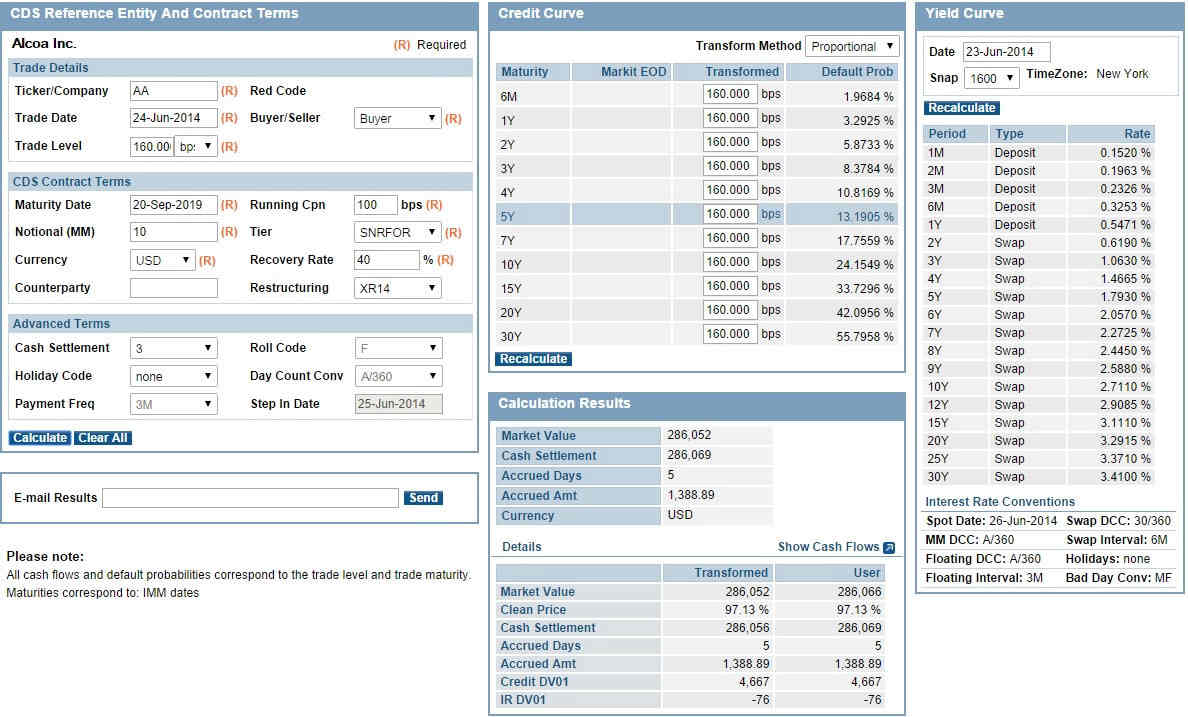
\includegraphics[width=6in]{MarkitCDSAlcoa.jpeg}
\caption{CDS figures from Markit.com}
\end{figure}

\begin{figure}[ht!]
\centering
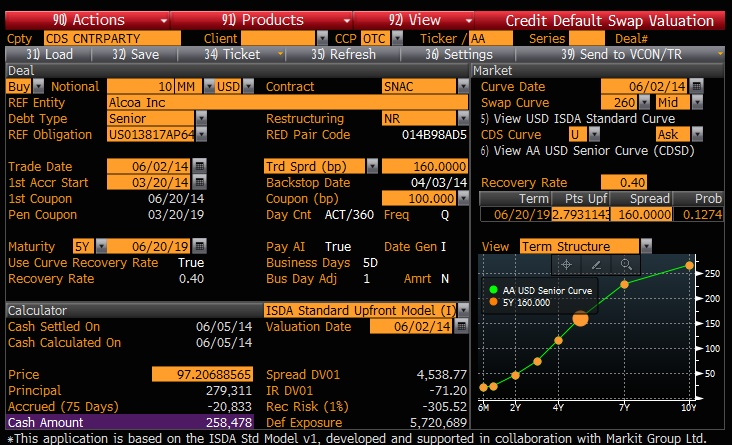
\includegraphics[width=6in]{BloombergCDSAlcoa.jpeg}
\caption{CDS figures from Bloomberg}
\end{figure}

\begin{figure}[ht!]
\centering
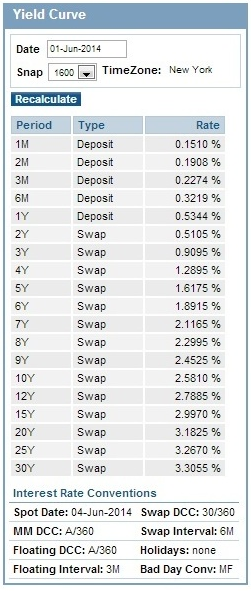
\includegraphics[width=6in]{MarkitIRJun2.jpeg}
\caption{Interest Rate figures from Markit.com}
\end{figure}

\begin{figure}[ht!]
\centering
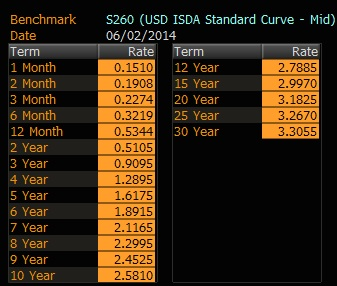
\includegraphics[width=6in]{BloombergIRJun2.jpeg}
\caption{Interest Rate figures from Bloomberg}
\end{figure}


\section{Conclusion}

In this paper, we describe the basics of a CDS contract and the ISDA
Standard Model. We also provide a simple collection
of tools to implement the Standard Model in \textbf{R} with the
\texttt{CDS} package. Moreover, the flexibility of \textbf{R} itself
allows users to extend and modify this package to suit their own
needs and/or create their preferred models for valuing CDS contracts. An
\textbf{R} package, \texttt{backtest} \cite{kane:david}, provides
facilities to explore portfolio-based conjectures about credit default
swaps. It is possible to use the \texttt{backtest} package based on
the output from the \texttt{CDS} package. Before reaching that level
of complexity, however, \texttt{CDS} provides a good starting point
for valuing credit default swaps.


\bibliography{CDS}



\end{document}


